\section{ontwerp}
In dit hoofdstuk wordt het ontwerp van het sensor fusion systeem beschreven. Op basis van het vooronderzoek en de vastgestelde specificaties zijn de ontwerpkeuzes gemaakt die in dit hoofdstuk worden toegelicht. Het hoofdstuk begint met een beschrijving van de bestaande hardware van de MYLAPS RTK tracker, gevolgd door de systeemarchitectuur en tot slot het wiskundig ontwerp van het filter. Het doel van dit hoofdstuk is om de brug te slaan tussen het theoretisch kader en de uiteindelijke implementatie. 
\todo[inline]{Inleiding aanpassen}

\subsection{Het huidige systeem}

Het sensor fusion systeem wordt geïmplementeerd op de bestaande MYLAPS ProRTK tracker. Voordat het ontwerp van het systeem wordt beschreven, is het relevant het huidige systeem van de tracker in kaart te brengen. De ProRTK is een compacte, herlaadbare sporttimer die draadloos communiceert met de MYLAPS server via het X2 Link protocol. Het apparaat combineert een RTK GNSS-ontvanger met een IMU op één printplaat. De voor dit project relevante hardwarecomponenten zijn weergegeven in tabel \ref{tab:hardware}.

\begin{table}[htbp]
    \centering
    \caption{Relevante hardwarecomponenten van de MYLAPS ProRTK tracker.}
    \label{tab:hardware}
    \renewcommand{\arraystretch}{1.3}
    \begin{tabularx}{\textwidth}{|l|X|X|}
        \hline
        \rowcolor{green!20}
        \textbf{Component} & \textbf{Type} & \textbf{Functie} \\ \hline
        Microcontroller &
        Nordic Semiconductor nRF52, ARM Cortex-M4F \cite{nordic_nrf52832_ps} &
        Verwerkt alle data en draait het gehele systeem \\ \hline
        GNSS-ontvanger &
        u-blox X20P RTK ontvanger &
        Levert RTK positie en bijbehorende data (bijvoorbeeld snelheid) op 25 Hz 
        via UART \\ \hline
        IMU &
        STMicroelectronics ASM330LHH, 6-assig &
        Levert versnelling en hoeksnelheid op 200 Hz 
        via SPI \\ \hline
        Seriële flash &
        Externe NOR-flash &
        Opslag van logs en instellingen, gedeelde SPI-bus \\ \hline
        CAN-controller &
        CAN-bus interface &
        Communicatie met timinginfrastructuur, 
        gedeelde SPI-bus \\ \hline
    \end{tabularx}
\end{table}

Het gehele systeem van de tracker wordt aangestuurd door de nRF52832 microcontroller met een ARM Cortex-M4F processor. Deze is verantwoordelijk voor het verwerken van de GNSS data uit de ublox module en de communicatie met de IMU. Een belangrijk onderdeel van deze microcontroller is de beschikbare Floating-Point Unit (FPU). Aangezien het filter gebruik zal maken van veel wiskundig complexe berekeningen, is het noodzakelijk dat de software dit kan afhandelen zonder vertragingen. \\

De locatiebepaling wordt doormiddel van de u-blox X20P RTK ontvanger tot stand gebracht. 

De locatiebepaling wordt primair gevoed door de u-blox X20P RTK-ontvanger. In tegenstelling tot standaard GPS-modules, levert deze ontvanger via de UART-verbinding niet alleen de actuele positie en snelheid op 25 Hz, maar verstrekt deze ook gedetailleerde onzekerheidsmarges (covarianties). Deze stroom aan extra diagnostische data is van enorme waarde voor het filterontwerp, maar vereist efficiënte communicatie via de UART-bus om vertragingen te voorkomen.  De interne bewegingsdynamiek wordt geregistreerd door de STMicroelectronics ASM330LHH. Dit is een 6-assige, automotive-grade IMU die versnellingen en hoeksnelheden aanlevert met een geconfigureerde frequentie van 200 Hz. 


Een belangrijke architecturale uitdaging van de ProRTK-hardware is dat de communicatie met deze IMU via een Serial Peripheral Interface (SPI) verloopt, waarbij de fysieke bus wordt gedeeld met de externe NOR-flash (voor dichte datalogging) en de CAN-controller (voor voertuigtelemetrie). Dit gedeelde hardware-design vormt een fysieke bottleneck. Het uitlezen van de sensordata op 200 Hz moet in het software-ontwerp dan ook strikt gesynchroniseerd worden middels hardware-interrupts (Chip Select), om te voorkomen dat data-corruptie optreedt wanneer de IMU actief wordt uitgelezen terwijl de processor gelijktijdig bezig is met het wegschrijven van logs naar de flash-opslag. 

\newpage

\subsection{Black box}

\begin{figure}[htbp]
\centering
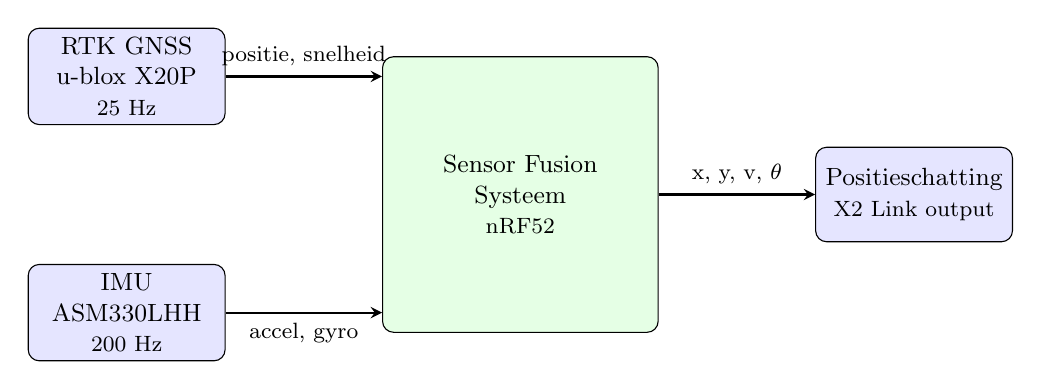
\begin{tikzpicture}[
    block/.style={rectangle, draw, rounded corners=4pt,
              minimum width=3cm, minimum height=1.2cm,
              text centered, align=center,
              fill=blue!10, font=\small},
    smallblock/.style={rectangle, draw, rounded corners=3pt,
              minimum width=2.2cm, minimum height=0.9cm,
              text centered, align=center,
              fill=orange!15, font=\footnotesize},
    decision/.style={diamond, draw, fill=yellow!20,
              minimum width=2.5cm, minimum height=1cm,
              text centered, align=center,
              font=\footnotesize, aspect=2},
    arrow/.style={->, thick, >=stealth}
]
    \node[block, minimum width=2.5cm] (gps)  at (0, 1.5)
        {RTK GNSS\\u-blox X20P\\{\footnotesize 25 Hz}};
    \node[block, minimum width=2.5cm] (imu)  at (0, -1.5)
        {IMU\\ASM330LHH\\{\footnotesize 200 Hz}};
    \node[block, minimum width=3.5cm, minimum height=3.5cm,
          fill=green!10] (sf) at (5, 0)
        {Sensor Fusion\\Systeem\\{\footnotesize nRF52}};
    \node[block, minimum width=2.5cm] (out) at (10, 0)
        {Positieschatting\\{\footnotesize X2 Link output}};

    \draw[arrow] (gps.east) -- node[above, font=\footnotesize]
        {positie, snelheid} (sf.west |- gps.east);
    \draw[arrow] (imu.east) -- node[below, font=\footnotesize]
        {accel, gyro} (sf.west |- imu.east);
    \draw[arrow] (sf.east) -- node[above, font=\footnotesize]
        {x, y, v, $\theta$} (out.west);
\end{tikzpicture}
\caption{\textbf{Niveau 1 -- Blackbox overzicht:} het sensor fusion systeem
ontvangt twee asynchrone datastromen en levert één betrouwbare
positieschatting via het X2 Link protocol.}
\label{fig:blackbox}
\end{figure}


\subsection{Interne architectuur}

\begin{figure}[htbp]
\centering
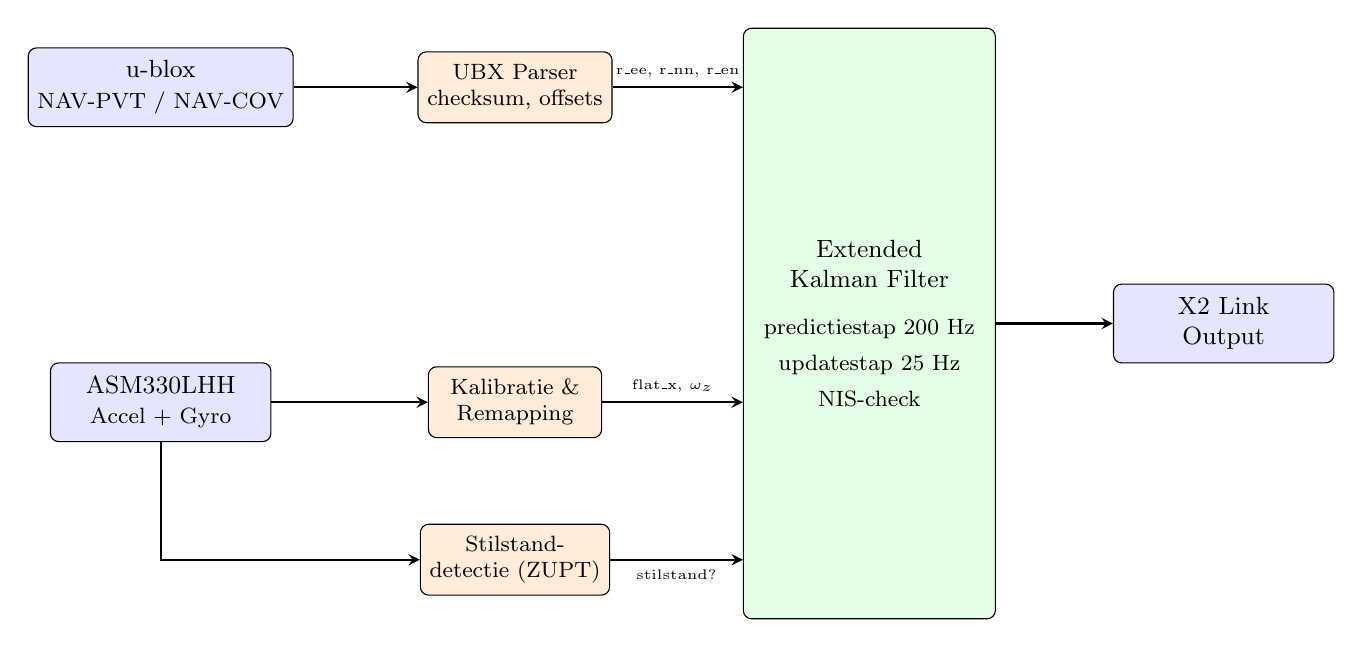
\begin{tikzpicture}[
    block/.style={rectangle, draw, rounded corners=3pt,
                  minimum width=2.8cm, minimum height=1cm,
                  text centered, align=center,
                  fill=blue!10, font=\small},
    smallblock/.style={rectangle, draw, rounded corners=3pt,
                  minimum width=2.2cm, minimum height=0.9cm,
                  text centered, align=center,
                  fill=orange!15, font=\footnotesize},
    arrow/.style={->, thick, >=stealth}
]
    \node[block] (gps) at (0, 3)
        {u-blox\\{\footnotesize NAV-PVT / NAV-COV}};
    \node[block] (imu) at (0, -1)
        {ASM330LHH\\{\footnotesize Accel + Gyro}};

    \node[smallblock] (parser) at (4.5, 3)
        {UBX Parser\\{\footnotesize checksum, offsets}};
    \node[smallblock] (cal)    at (4.5, -1)
        {Kalibratie \&\\Remapping};
    \node[smallblock] (zupt)   at (4.5, -3)
        {Stilstand-\\detectie (ZUPT)};

    \node[block, minimum width=3.2cm, minimum height=7.5cm,
        fill=green!10] (ekf) at (9, 0)
        {Extended\\Kalman Filter\\[6pt]
        {\footnotesize predictiestap 200 Hz}\\[2pt]
        {\footnotesize updatestap 25 Hz}\\[2pt]
        {\footnotesize NIS-check}};

    \node[block] (out) at (13.5, 0)
        {X2 Link\\Output};

    % GPS naar parser
    \draw[arrow] (gps) -- (parser);

    % IMU naar kalibratie en ZUPT
    \draw[arrow] (imu) -- (cal);
    \draw[arrow] (imu) |- (zupt);

    % Parser naar EKF: horizontale lijn op hoogte van parser
    \draw[arrow] (parser.east) --
        node[above, font=\tiny] {r\_ee, r\_nn, r\_en}
        (ekf.west |- parser.east);

    % Kalibratie naar EKF: horizontale lijn op hoogte van cal
    \draw[arrow] (cal.east) --
        node[above, font=\tiny] {flat\_x, $\omega_z$}
        (ekf.west |- cal.east);

    % ZUPT naar EKF: horizontale lijn op hoogte van zupt
    \draw[arrow] (zupt.east) --
        node[below, font=\tiny] {stilstand?}
        (ekf.west |- zupt.east);

    % EKF naar output
    \draw[arrow] (ekf) -- (out);

\end{tikzpicture}
\caption{\textbf{Niveau 2 -- Interne architectuur:} de twee datastromen worden
voorverwerkt voordat zij de EKF bereiken. De EKF voert op 200 Hz
de predictiestap uit en op 25 Hz de updatestap met NIS-check.}
\label{fig:architectuur}
\end{figure}

\newpage


\subsection{EKF dataflow}

\begin{figure}[htbp]
\centering
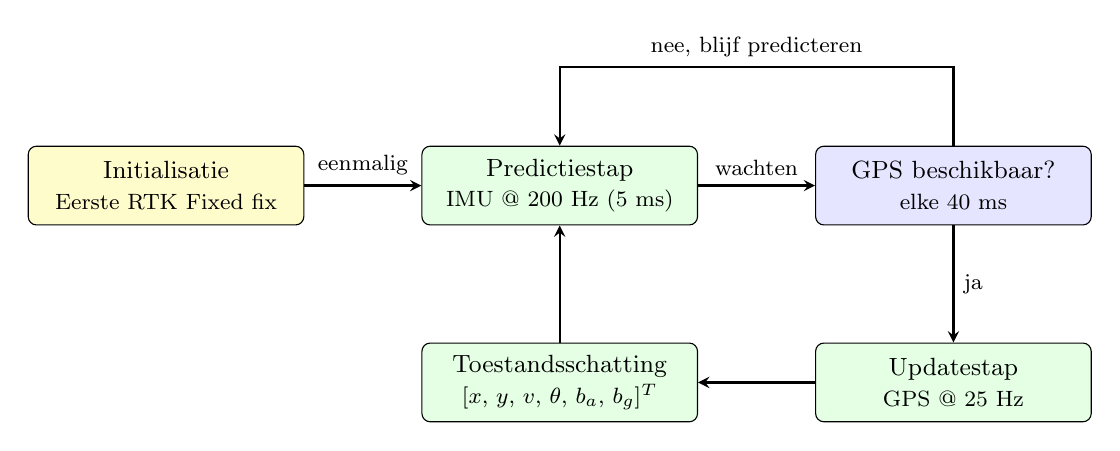
\begin{tikzpicture}[
    block/.style={rectangle, draw, rounded corners=3pt,
                  minimum width=3.5cm, minimum height=1cm,
                  text centered, align=center,
                  fill=blue!10, font=\small},
    blockgreen/.style={rectangle, draw, rounded corners=3pt,
                  minimum width=3.5cm, minimum height=1cm,
                  text centered, align=center,
                  fill=green!10, font=\small},
    blockyellow/.style={rectangle, draw, rounded corners=3pt,
                  minimum width=3.5cm, minimum height=1cm,
                  text centered, align=center,
                  fill=yellow!20, font=\small},
    arrow/.style={->, thick, >=stealth}
]
    % Initialisatie
    \node[blockyellow] (init) at (0, 0)
        {Initialisatie\\{\footnotesize Eerste RTK Fixed fix}};

    % Predictiestap
    \node[blockgreen] (pred) at (5, 0)
        {Predictiestap\\{\footnotesize IMU @ 200 Hz (5 ms)}};

    % GPS check
    \node[block] (gps) at (10, 0)
        {GPS beschikbaar?\\{\footnotesize elke 40 ms}};

    % Updatestap
    \node[blockgreen] (upd) at (10, -2.5)
        {Updatestap\\{\footnotesize GPS @ 25 Hz}};

    % Uitvoer
    \node[blockgreen] (out) at (5, -2.5)
        {Toestandsschatting\\
         {\footnotesize $[x,\, y,\, v,\, \theta,\, b_a,\, b_g]^T$}};

    % Pijlen
    \draw[arrow] (init) -- node[above, font=\footnotesize]
        {eenmalig} (pred);
    \draw[arrow] (pred) -- node[above, font=\footnotesize]
        {wachten} (gps);
    \draw[arrow] (gps)  -- node[right, font=\footnotesize]
        {ja} (upd);
    \draw[arrow] (gps.north) -- ++(0, 1)
        -- node[above, font=\footnotesize] {nee, blijf predicteren}
        ++(-5, 0) -- (pred.north);
    \draw[arrow] (upd)  -- (out);
    \draw[arrow] (out)  -- (pred);

\end{tikzpicture}
\caption{Flowchart van het algoritme na een eenmalige initialisatie
bij de eerste RTK Fixed fix draait de predictiestap continu op 200 Hz.
Elke 40 ms wordt een GPS-meting verwerkt in de updatestap waarna
de toestandsschatting wordt bijgewerkt.}
\label{fig:ekf_flow}
\end{figure}


\newpage